\section{Рабочий проект}

\subsection{Спецификация компонентов и классов программной системы}

\subsubsection{Спецификация поискового робота}

Поисковый робот имеет собственный конфигурационный файл "<crawler.yaml"> в формате YAML для описания различного рода настроек. Приведем его описание:
\begin{itemize}
\item component\_name -- название компонента в рамках распределенной поисковой системы;
\item name -- имя робота в сети Интернет;
\item services -- опции, непосредственно связанные с сервисами робота:
\begin{itemize}
\item distributor -- опции, связанные с работой сервиса распределения ресурсов:
\begin{itemize}
\item thread\_pool -- размер пула потоков;
\item domain\_group\_size -- размер рабочей группы доменов, ресурсы из базы данных которых в первую очередь обрабатываются;
\item max\_pages\_batch\_size -- максимальное количество страниц, которые берутся из базы данных для дальнейшей обработки в рамках одного доменного имени за одну операцию;
\item interval\_ms -- интервал времени в миллисекундах, который проходит между операциями считывания новых ресурсов из базы данных для обработки.
\end{itemize}
\item queue -- опции, связанные с работой сервиса хранения ресурсов:
\begin{itemize}
\item thread\_pool -- размер пула потоков;
\item group\_fetch\_delay\_ms -- минимальная задержка в миллисекундах между последовательным сбором ресурсов из одного внешнего источника;
\item max\_size -- максимальный размер очереди хранения.
\end{itemize}
\item processor -- опции, связанные с работой сервиса обработки ресурсов:
\begin{itemize}
\item thread\_pool -- размер пула потоков;
\item max\_size -- максимальное количество одновременно открытых файловых дескрипторов для сбора ресурсов из внешних источников;
\item max\_resource\_size -- максимальный размер ресурса в байтах для обработки;
\item fetch\_resource\_timeout\_ms -- максимальное время ожидания получения ресурса из внешнего источника в миллисекундах.
\end{itemize}
\end{itemize}
\item db -- опции, связанные с взаимодействием c базой данных:
\begin{itemize}
\item pool\_size -- размер пула соединений к базе данных;
\item connection\_string -- строка подключения к базе данных.
\end{itemize}
\item bus -- опции, связанные с взаимодействием с шиной данных:
\begin{itemize}
\item pool\_size -- размер пула соединений к шине данных;
\item thread\_pool -- размер пула потоков;
\item connection\_string -- строка подключения к шине данных;
\item messages -- список типов сообщений, отправляемых на шину данных:
\begin{itemize}
\item name -- название сообщения;
\item enabled -- доступно ли для отправления;
\item exchange -- название удаленного приёмника сообщения;
\item routing\_key -- название ключа, определяющего очередь назначения сообщения;
\item max\_batch\_size -- максимальное количество экземпляров данных в одном сообщении;
\item max\_batch\_volume -- максимальный размер памяти, отведенный на одно сообщение;
\item compression\_type -- тип сжатия сообщения.
\end{itemize}
\end{itemize}
\item logging -- опции работы с журналируемыми сообщениями робота:
\begin{itemize}
\item lvl -- уровень логгирования;
\item log\_formats -- форматы вывода сообщений;
\item time\_formats -- форматы вывода дат сообщений.
\end{itemize}
\end{itemize}

Класс "<Config"> используется для хранения и оперативного получения данных из конфигурационного файла робота в формате YAML. В таблицах 4.1, 4.2 приведено описание полей и методов данного класса.
\begin{xltabular}{\textwidth}{|X|X|X|X|}
	\caption{Спецификация полей класса "<Config">}\label{robot_config_fields:table} \\ \hline
	\thead{Наименование} & \thead{Модификатор\\доступа}  & \thead{Тип\\данных} & \thead{Описание} \\ \hline
	\thead{1} & \thead{2} & \thead{3} & \thead{4} \\ \hline
	\endfirsthead
	\continuecaption{Продолжение таблицы \ref{robot_config_fields:table}} \hline
	\thead{1} & \thead{2} & \thead{3} & \thead{4} \\ \hline
	\endhead
	name & private & string & Имя робота \\ \hline
\end{xltabular}
\begin{xltabular}{\textwidth}{|X|X|X|}
	\caption{Спецификация методов класса "<Config">}\label{robot_config_methods:table} \\ \hline
	\thead{Наименование} & \thead{Модификатор\\доступа} & \thead{Описание} \\ \hline
	\thead{1} & \thead{2} & \thead{3} \\ \hline
	\endfirsthead
	\continuecaption{Продолжение таблицы \ref{robot_config_methods:table}} \hline
	\thead{1} & \thead{2} & \thead{3} \\ \hline
	\endhead
	name & public & Возвращает название робота \\ \hline
	max\_resource\_size & public & Возвращает максимальный допустимый размер ресурса \\ \hline
	from\_bus\_message & public & Возвращает значение опции отправки сообщения на шину. Аргументы: key -- название опции, path -- путь описания сообщений в конфигурационном файле. \\ \hline
	from\_service & public & Возвращает значение опции какого-либо внутреннего сервиса робота. Аргументы: key -- название опции, path -- путь описания опций сервиса. \\ \hline
	db\_config & public & Возвращает информацию по подключению к СУБД. \\ \hline
	init\_cached\_data & private & Инициализирует закешированные значения конфигурации для быстрого обращения в ходе исполнения. \\ \hline
\end{xltabular}

Класс "<Crawler"> используется как фасад для запуска поискового робота и его основных сервисов. В таблицах 4.3, 4.4 приведено описание полей и методов данного класса.
\begin{xltabular}{\textwidth}{|X|X|X|X|}
	\caption{Спецификация полей класса "<Crawler">}\label{robot_crawler_fields:table} \\ \hline
	\thead{Наименование} & \thead{Модификатор\\доступа} & \thead{Тип\\данных} & \thead{Описание} \\ \hline
	\thead{1} & \thead{2} & \thead{3} & \thead{4} \\ \hline
	\endfirsthead
	\continuecaption{Продолжение таблицы \ref{robot_crawler_fields:table}} \hline
	\thead{1} & \thead{2} & \thead{3} & \thead{4} \\ \hline
	\endhead
	config\_errors & private & atomic\_bool & Истинно, если процесс настройки сервисов завершился с ошибкой. \\ \hline
	distributor & private & Resource
	Distributor* & Указатель на сервис распределения ресурсов. \\ \hline
	processor & private & Resource
	Processor* & Указатель на сервис обработки ресурсов. \\ \hline
	queue & private & Resource
	Repository* & Указатель на сервис хранения и выдачи ресурсов для обработки. \\ \hline
	db & private & Postgres
	DataProvider* & Указатель на сервис управления данными из СУБД Postgres. \\ \hline
	bus & private & AMQPBus
	Mixin* & Указатель на сервис управления доступом к шине данных RabbitMQ, \\ \hline
	bus\_group & private & thread\_group & Пул потоков для сервиса шины. \\ \hline
	distributor\_
	group & private & thread\_group & Пул потоков для сервиса распределения. \\ \hline
	queue\_
	group & private & thread\_group & Пул потоков для сервиса хранения ресурсов. \\ \hline
	processor\_
	group & private & thread\_group & Пул потоков для сервиса обработки. \\ \hline
\end{xltabular}
\begin{xltabular}{\textwidth}{|X|X|X|}
	\caption{Спецификация методов класса "<Crawler">}\label{robot_crawler_methods:table} \\ \hline
	\thead{Наименование} & \thead{Модификатор\\доступа} & \thead{Описание} \\ \hline
	\thead{1} & \thead{2} & \thead{3} \\ \hline
	\endfirsthead
	\continuecaption{Продолжение таблицы \ref{robot_crawler_methods:table}} \hline
	\thead{1} & \thead{2} & \thead{3} \\ \hline
	\endhead
	setup & public & Проводит настройку всех внутренних сервисов. \\ \hline
	run & public & Запускает поискового робота. \\ \hline
	stop & public & Останавливает поискового робота. \\ \hline
	try\_configure\_db & private & Конфигурирует сервис базы данных. В случае успеха возвращает "<true">. \\ \hline
	try\_configure\_bus & private & Конфигурирует сервис шины данных. В случае успеха возвращает "<true">. \\ \hline
	try\_configure\_
	queue & private & Конфигурирует сервис хранения ресурсов. В случае успеха возвращает "<true">. \\ \hline
	try\_configure\_
	distributor & private & Конфигурирует сервис распределения ресурсов. В случае успеха возвращает "<true">. \\ \hline
	try\_configure\_
	processor & private & Конфигурирует сервис обработки ресурсов. В случае успеха возвращает "<true">. \\ \hline
	try\_configure\_
	logging & private & Конфигурирует сервис журналирования. В случае успеха возвращает "<true">. \\ \hline
\end{xltabular}

Класс "<ResourceDistributor"> используется для распределения ресурсов в очередь хранения. Ресурсы могут поступать как из процессора обработки ресурсов, так и из базы данных. В таблицах 4.5, 4.6 приведено описание полей и методов данного класса.
\begin{xltabular}{\textwidth}{|X|X|X|X|}
	\caption{Спецификация полей класса "<ResourceDistributor">}\label{robot_distributor_fields:table} \\ \hline
	\thead{Наименование} & \thead{Модификатор\\доступа} & \thead{Тип\\данных} & \thead{Описание} \\ \hline
	\thead{1} & \thead{2} & \thead{3} & \thead{4} \\ \hline
	\endfirsthead
	\continuecaption{Продолжение таблицы \ref{robot_distributor_fields:table}} \hline
	\thead{1} & \thead{2} & \thead{3} & \thead{4} \\ \hline
	\endhead
	group\_size & private & size\_t & Размер группы одновременно обрабатываемых доменов с ресурсами. \\ \hline
	max\_pages\_batch\_size & private & size\_t & Размер группы ресурсов для обработки. \\ \hline
	async\_count & private & atomic\_size\_t & Количество текущих асинхронных операций. \\ \hline
	data & private & IDataProvider* & Указатель на реализацию интерфейса сервиса для работы с СУБД. \\ \hline
	repository & private & ResourcesRepository* & Указатель на сервис хранения ресурсов. \\ \hline
	resolver & private & ResourceLoader & Асинхронный сопоставитель доменному имени IPv4 адреса. \\ \hline
	headers & private & CrawlingHeadersContainer & Lock-free хеш-таблица для хранения информации о текущих заголовках ресурсов по доменному имени. \\ \hline
	used\_resources & private & UsedResourcesContainer & Lock-free множество ресурсов, обработка которых еще не закончена. \\ \hline
\end{xltabular}
\begin{xltabular}{\textwidth}{|X|X|X|}
	\caption{Спецификация методов класса "<ResourceDistributor">}\label{robot_distributor_methods:table} \\ \hline
	\thead{Наименование} & \thead{Модификатор\\доступа} & \thead{Описание} \\ \hline
	\thead{1} & \thead{2} & \thead{3} \\ \hline
	\endfirsthead
	\continuecaption{Продолжение таблицы \ref{robot_distributor_methods:table}} \hline
	\thead{1} & \thead{2} & \thead{3} \\ \hline
	\endhead
	run & public & Запускает распределитель. \\ \hline
	size & public & Возвращает количество текущих асинхронных операций. \\ \hline
	current\_crawling\_
	group\_size & public & Возвращает текущий размер рабочей группы доменов. \\ \hline
	distribute & public & Синхронно распределяет ресурс в очередь хранения. Аргументы: resource -- указатель на ресурс. \\ \hline
	distribute\_nowait & public & Асинхронно распределяет коллекцию ресурсов в очередь хранения. Аргументы: resources -- коллекция ресурсов. \\ \hline
	mark\_as\_handled & public & Помечает ресурс как обработанный и удаляет его из множества необработанных. Аргументы: resource -- указатель на ресурс. \\ \hline
	distribute\_some\_
	from\_header & private & Выбирает некоторое количество необработанных ресурсов из базы данных для заданного доменного имени и передает их в очередь хранения для обработки. Аргументы: name -- доменное имя. \\ \hline
	remove\_crawled\_headers & private & Удаляет из хеш-таблицы доменные имена, ресурсы которых были полностью обработаны. \\ \hline
	add\_new\_headers & private & Добавляет новые доменные имена в хеш-таблицу для добавления их ресурсов в очередь хранения. \\ \hline
	distribute\_no\_check & private & Распределяет ресурс в очередь хранения без каких-либо проверок. Аргументы: resource -- указатель на ресурс. \\ \hline
\end{xltabular}

Класс "<ResourcesRepository"> используется для хранения очередей ресурсов. Каждая очередь ассоциирована с некоторым IP адресом. Сделано это для того, чтобы на один и тот же IP адрес не поступали запросы в некоторый фиксированный временной интервал, чтобы внешние сервера не интерпретировали это как DDOS-атаку [49]. В таблицах 4.7, 4.8 приведено описание полей и методов данного класса.
\begin{xltabular}{\textwidth}{|X|X|X|X|}
	\caption{Спецификация полей класса "<ResourcesRepository">}\label{robot_repository_fields:table} \\ \hline
	\thead{Наименование} & \thead{Модификатор\\доступа} & \thead{Тип\\данных} & \thead{Описание} \\ \hline
	\thead{1} & \thead{2} & \thead{3} & \thead{4} \\ \hline
	\endfirsthead
	\continuecaption{Продолжение таблицы \ref{robot_repository_fields:table}} \hline
	\thead{1} & \thead{2} & \thead{3} & \thead{4} \\ \hline
	\endhead
	max\_resources
	\_count & private & size\_t & Максимальное количество ресурсов в очереди хранения. \\ \hline
	group\_fetch\_
	delay\_ms & private & milliseconds & Задержка отправки ресурса в выходную очередь после получения сигнала о сделанном запросе. \\ \hline
	count & private & atomic\_size\_t & Текущее количество ресурсов в очереди. \\ \hline
	free\_space\_
	notifier & private & AsyncEvent & Асинхронная условная переменная для уведомления потоков о появившемся свободном месте в очереди хранения. \\ \hline
	output\_queue & private & FCPriorityQueue & Выходная очередь ресурсов. \\ \hline
	groups & private & GroupsContainer & Lock-free хеш-таблица для хранения очередей с приорететами ресурсов в отдельности для каждого IPv4 адреса. \\ \hline
\end{xltabular}
\begin{xltabular}{\textwidth}{|X|X|X|}
	\caption{Спецификация методов класса "<ResourcesRepository">}\label{robot_repository_methods:table} \\ \hline
	\thead{Наименование} & \thead{Модификатор\\доступа} & \thead{Описание} \\ \hline
	\thead{1} & \thead{2} & \thead{3} \\ \hline
	\endfirsthead
	\continuecaption{Продолжение таблицы \ref{robot_repository_methods:table}} \hline
	\thead{1} & \thead{2} & \thead{3} \\ \hline
	\endhead
	run & public & Запускает очередь хранения. \\ \hline
	size & public & Возвращает общее количество ресурсов в очереди. \\ \hline
	output\_size & public & Возвращает количество ресурсов в выходной очереди. \\ \hline
	group\_size & public & Возвращает количество групп ресурсов. \\ \hline
	is\_full & public & Возвращает ответ на запрос, полна ли очередь. \\ \hline
	push & public & Добавляет ресурс в очередь. Аргументы: group\_name -- название целевой группы, resource -- указатель на ресурс. \\ \hline
	try\_pop & public & Делает попытку вернуть ресурс из выходной очереди. Возвращает "<true"> в случае успеха. Аргументы: resource -- ссылка на возвращаемый ресурс. \\ \hline
	reload\_group & public & Выполняет перезагрузку целевой очереди. По её окончании наиболее приоритетный ресурс будет размещен в выходной очереди. \\ \hline
	reset & public & Выполняет полный сброс текущего состояния очереди хранения. \\ \hline
	handle\_expired\_reload & private & Обработчик окончания перезагрузки группы ресурсов. Аргументы: group\_name -- название группы. \\ \hline
	push\_impl & private & Внутренняя общая реал 
изация добавления ресурса в очередь хранения. Аргументы: group\_name -- название группы, resource -- указатель на ресурс, output -- флаг, уточняющий направление добавления ресурса. \\ \hline
	push\_with\_overflow & private & Реализация добавления ресурса при переполнении очереди. Аргументы: resource -- указатель на ресурс, state -- указатель на структуру группы ресурсов. \\ \hline
	push\_to\_output & private & Отправляет ресурс непосредственно в выходную очередь. Аргументы: resource -- указатель на ресурс. \\ \hline
\end{xltabular}

Класс "<ResourceProcessor"> используется для обработки поступающих ресурсов. Именно в этом компоненте одни ресурсы могут порождать множество других и дальнейшее их распределение процессор возлагает на ранее рассмотренный "<ResourceDistributor"> [50]. В таблицах 4.9, 4.10 приведено описание полей и методов данного класса.
\begin{xltabular}{\textwidth}{|X|X|X|X|}
	\caption{Спецификация полей класса "<ResourceProcessor">}\label{robot_processor_fields:table} \\ \hline
	\thead{Наименование} & \thead{Модификатор\\доступа} & \thead{Тип\\данных} & \thead{Описание} \\ \hline
	\thead{1} & \thead{2} & \thead{3} & \thead{4} \\ \hline
	\endfirsthead
	\continuecaption{Продолжение таблицы \ref{robot_processor_fields:table}} \hline
	\thead{1} & \thead{2} & \thead{3} & \thead{4} \\ \hline
	\endhead
	max\_concurrent\_
	handlers\_count & private & size\_t & Максимальное количество одновременно работающих обработчиков. \\ \hline
	total\_handled & private & atomic\_size\_t & Общее количество обработанных ресурсов. \\ \hline
	total\_succeed\_handled & private & atomic\_size\_t & Общее количество успешно обработанных ресурсов. \\ \hline
	total\_in\_work & private & atomic\_size\_t & Количество обрабатываемых ресурсов в данный момент времени. \\ \hline
	distributor & private & Resource
	Distributor* & Указатель на сервис распределения ресурсов. \\ \hline
	repository & private & Resources
	Repository* & Указатель на сервис хранения ресурсов. \\ \hline
	db & private & IDataProvider* & Указатель на сервис управления доступом к данным СУБД. \\ \hline
	bus & private & IExternalBus* & Указатель на шину данных. \\ \hline
\end{xltabular}
\begin{xltabular}{\textwidth}{|X|X|X|}
	\caption{Спецификация методов класса "<ResourceProcessor">}\label{robot_processor_methods:table} \\ \hline
	\thead{Наименование} & \thead{Модификатор\\доступа} & \thead{Описание} \\ \hline
	\thead{1} & \thead{2} & \thead{3} \\ \hline
	\endfirsthead
	\continuecaption{Продолжение таблицы \ref{robot_processor_methods:table}} \hline
	\thead{1} & \thead{2} & \thead{3} \\ \hline
	\endhead
	run & public & Запускает процессор по обработке ресурсов. \\ \hline
	total\_handled & public & Возвращает общее количество обработанных ресурсов. \\ \hline
	total\_succeed\_handled & public & Возвращает общее количество успешно обработанных ресурсов. \\ \hline
	total\_in\_work & public & Возвращает текущее количество ресурсов в обработке. \\ \hline
	handle\_resource\_
	received & public & Обрабатывает событие получения удаленного ресурса. Аргументы: resource -- указатель на ресурс, success -- флаг успешности получения, retry\_delay -- требуемая задержка для следующего запроса. \\ \hline
	handle\_new\_resources & public & Обрабатывает событие появления новых ресурсов для обработки. Аргументы: resources -- коллекция ресурсов. \\ \hline
	commit\_resource & public & Обрабатывает событие подтверждения нового индексируемого ресурса. Аргументы: resource -- указатель на индексируемый ресурс. \\ \hline
	send\_to\_index & public & Отправляет информацию об обработанном ресурсе на сервис шины данных. \\ \hline
	on\_handling\_end & public & Обрабатывает событие окончания обработки ресурса. \\ \hline
\end{xltabular}

Класс "<PostgresDataProvider"> используется в качестве адаптера для работы с базой данных. Он реализует интерфейс, который необходим другим компонентам, которые взаимодействуют с СУБД Postgres. В таблицах 4.11, 4.12 приведено описание полей и методов данного класса.
\begin{xltabular}{\textwidth}{|X|X|X|X|}
	\caption{Спецификация полей класса "<PostgresDataProvider">}\label{robot_data_provider_fields:table} \\ \hline
	\thead{Наименование} & \thead{Модификатор\\доступа} & \thead{Тип\\данных} & \thead{Описание} \\ \hline
	\thead{1} & \thead{2} & \thead{3} & \thead{4} \\ \hline
	\endfirsthead
	\continuecaption{Продолжение таблицы \ref{robot_data_provider_fields:table}} \hline
	\thead{1} & \thead{2} & \thead{3} & \thead{4} \\ \hline
	\endhead
	config & private & DbConfig & Данные конфигурации для работы с СУБД. \\ \hline
	connections & private & Postgres
	ConnectionsPool & Пул соединений для работы с СУБД. \\ \hline
\end{xltabular}
\begin{xltabular}{\textwidth}{|X|X|X|}
	\caption{Спецификация методов класса "<PostgresDataProvider">}\label{robot_data_provider_methods:table} \\ \hline
	\thead{Наименование} & \thead{Модификатор\\доступа} & \thead{Описание} \\ \hline
	\thead{1} & \thead{2} & \thead{3} \\ \hline
	\endfirsthead
	\continuecaption{Продолжение таблицы \ref{robot_data_provider_methods:table}} \hline
	\thead{1} & \thead{2} & \thead{3} \\ \hline
	\endhead
	enabled & public & Возвращает "<true"> в случае валидного открытого подключения к СУБД. \\ \hline
	get\_unhandled\_
	headers\_top & public & Возвращает коллекцию доменов с наибольшим числом необработанных ресурсов. Аргументы: limit -- максимальный размер коллекци. \\ \hline
	get\_unhandled\_top\_
	by\_header & public & Возвращает коллекцию ресурсов определенного домена с наибольшим приоритетом по убыванию. Аргументы: header -- доменное имя ресурса, limit -- максимальный размер коллекции. \\ \hline
	get\_resource & public & Возвращает указатель на ресурс из базы данных. Аргументы: header -- доменное имя ресурса, name -- название ресурса в рамках доменного имени. \\ \hline
	upload\_resource & public & Загружает информацию о ресурсе в базу данных. Аргументы: resource -- указатель на ресурс. \\ \hline
	finalize & public & Выполняет операции в базе данных по завершении обхода. \\ \hline
	validate\_connection & private & Производит валидацию подключения к базе данных. Аргументы: connection -- объект подключения к базе данных. \\ \hline
\end{xltabular}

Класс "<IExternalBus"> является адаптером для работы с шиной данных, в частности, с RabbitMQ. В таблицах 4.13, 4.14 приведено описание полей и методов данного класса.
\begin{xltabular}{\textwidth}{|X|X|X|X|}
	\caption{Спецификация полей класса "<IExternalBus">}\label{robot_bus_fields:table} \\ \hline
	\thead{Наименование} & \thead{Модификатор\\доступа} & \thead{Тип\\данных} & \thead{Описание} \\ \hline
	\thead{1} & \thead{2} & \thead{3} & \thead{4} \\ \hline
	\endfirsthead
	\continuecaption{Продолжение таблицы \ref{robot_bus_fields:table}} \hline
	\thead{1} & \thead{2} & \thead{3} & \thead{4} \\ \hline
	\endhead
	config & private & BusConfig & Конфигурация подключения к шине данных. \\ \hline
\end{xltabular}
\begin{xltabular}{\textwidth}{|X|X|X|}
	\caption{Спецификация методов класса "<IExternalBus">}\label{robot_bus_methods:table} \\ \hline
	\thead{Наименование} & \thead{Модификатор\\доступа} & \thead{Описание} \\ \hline
	\thead{1} & \thead{2} & \thead{3} \\ \hline
	\endfirsthead
	\continuecaption{Продолжение таблицы \ref{robot_bus_methods:table}} \hline
	\thead{1} & \thead{2} & \thead{3} \\ \hline
	\endhead
	send\_resource & public & Отправляет информацию об обработанном ресурсе на шину данных. Аргументы: data -- информация о ресурсе. \\ \hline
	send\_log & public & Отправляет журналируемую информацию на шину данных. Аргументы: data -- сведения из журнала. \\ \hline 
\end{xltabular}

\subsubsection{Спецификация индексатора}

Индексатор имеет собственный конфигурационный файл "<indexer.yaml"> в формате YAML для описания различного рода настроек. Приведем его описание:
\begin{itemize}
\item component\_name -- название компонента в рамках распределенной поисковой системы;
\item options -- опции, непосредственно связанные с вычислительными узлами индексатора:
\begin{itemize}
\item resources\_capacity -- необходимое количество обработанных ресурсов для начала следующих стадии индексирования, в ходе которых новые ресурсы перестанут считываться с шины данных;
\item loader -- опции загрузчика ресурсов из шины данных:
\begin{itemize}
\item batch\_size -- размер группы ресурсов для одной операции чтения из шины данных;
\item speed -- предполагаемая скорость первичной обработки ресурсов, выраженная в количестве ресурсов в секунду.
\end{itemize}
\item resources\_ranking -- опции вычисления статического ранга документов:
\begin{itemize}
\item teleport\_probability -- вероятность телепортации в результате случайного блуждания по веб-графу;
\item ranking\_iterations\_count -- количество итераций при вычислении левого собственного вектора матрицы вероятностных переходов веб-графа.
\end{itemize}
\item champion\_lists -- опции, связанные с формированием "<чемпионских"> списков:
\begin{itemize}
\item size -- максимальный размер списков;
\item threshold -- нижняя допустимая граница статического ранга лексемы в документе.
\end{itemize}
\item primary\_indexer -- опции по первичной обработке ресурсов:
\begin{itemize}
\item thread\_pool -- размер пула потоков;
\item compression\_type -- тип сжатия содержимого документов в базе данных;
\item min\_lexem\_size -- минимальная длина лексемы;
\item max\_lexem\_size -- максимальная длина лексемы;
\item tags -- опции обработки HTML-тегов:
\begin{itemize}
\item skip -- список тегов, которые не участвуют в анализе и будут удалены из содержимого документа;
\item weights -- абсолютные веса тегов документа для более точного вычисления абсолютного ранга вхождения термина в документ.
\end{itemize}
\end{itemize}
\end{itemize}
\item db -- опции, связанные с взаимодействием c базой данных:
\begin{itemize}
\item pool\_size -- размер пула соединений к базе данных;
\item connection\_string -- строка подключения к базе данных.
\end{itemize}
\item bus -- опции, связанные с взаимодействием с шиной данных:
\begin{itemize}
\item pool\_size -- размер пула соединений к шине данных;
\item thread\_pool -- размер пула потоков;
\item connection\_string -- строка подключения к шине данных;
\item queues -- список очередей, из которых происходит считывание данных;
\item messages -- список типов сообщений, отправляемых на шину данных:
\begin{itemize}
\item name -- название сообщения;
\item enabled -- доступно ли для отправления;
\item exchange -- название удаленного приёмника сообщения;
\item routing\_key -- название ключа, определяющего очередь назначения сообщения;
\item max\_batch\_size -- максимальное количество экземпляров данных в одном сообщении;
\item max\_batch\_volume -- максимальный размер памяти, отведенный на одно сообщение;
\item compression\_type -- тип сжатия сообщения.
\end{itemize}
\end{itemize}
\item logging -- опции работы с журналируемыми сообщениями робота:
\begin{itemize}
\item lvl -- уровень логгирования;
\item log\_formats -- форматы вывода сообщений;
\item time\_formats -- форматы вывода дат сообщений.
\end{itemize}
\end{itemize}

Класс "<Config"> используется для хранения и оперативного получения данных из конфигурационного файла индексатора в формате YAML. В таблице 4.15 приведено описание методов данного класса.
\begin{xltabular}{\textwidth}{|X|X|X|}
	\caption{Спецификация методов класса "<Config">}\label{indexer_config_methods:table} \\ \hline
	\thead{Наименование} & \thead{Модификатор\\доступа} & \thead{Описание} \\ \hline
	\thead{1} & \thead{2} & \thead{3} \\ \hline
	\endfirsthead
	\continuecaption{Продолжение таблицы \ref{indexer_config_methods:table}} \hline
	\thead{1} & \thead{2} & \thead{3} \\ \hline
	\endhead
	from\_bus\_message & public & Возвращает значение опции отправки сообщения на шину. Аргументы: key -- название опции, path -- путь описания сообщений в конфигурационном файле. \\ \hline
	options & public & Возвращает настройки индексирования. \\ \hline
	db\_config & public & Возвращает информацию по подключению к СУБД. \\ \hline
\end{xltabular}

Класс "<Indexer"> используется как фасад для запуска индексатора и его основных вычислительных компонентов. В таблицах 4.16, 4.17 приведено описание полей и методов данного класса.
\begin{xltabular}{\textwidth}{|X|X|X|X|}
	\caption{Спецификация полей класса "<Indexer">}\label{indexer_indexer_fields:table} \\ \hline
	\thead{Наименование} & \thead{Модификатор\\доступа} & \thead{Тип\\данных} & \thead{Описание} \\ \hline
	\thead{1} & \thead{2} & \thead{3} & \thead{4} \\ \hline
	\endfirsthead
	\continuecaption{Продолжение таблицы \ref{indexer_indexer_fields:table}} \hline
	\thead{1} & \thead{2} & \thead{3} & \thead{4} \\ \hline
	\endhead
	config\_errors & private & atomic\_bool & Истинно, если процесс настройки индексатора завершился с ошибкой. \\ \hline
	db & private & Postgres
	DataProvider* & Указатель на сервис управления данными из СУБД Postgres. \\ \hline
	bus & private & AMQPBus
	Mixin* & Указатель на сервис управления доступом к шине данных RabbitMQ, \\ \hline
	bus\_group & private & thread\_group & Пул потоков для сервиса шины. \\ \hline
\end{xltabular}
\begin{xltabular}{\textwidth}{|X|X|X|}
	\caption{Спецификация методов класса "<Indexer">}\label{indexer_indexer_methods:table} \\ \hline
	\thead{Наименование} & \thead{Модификатор\\доступа} & \thead{Описание} \\ \hline
	\thead{1} & \thead{2} & \thead{3} \\ \hline
	\endfirsthead
	\continuecaption{Продолжение таблицы \ref{indexer_indexer_methods:table}} \hline
	\thead{1} & \thead{2} & \thead{3} \\ \hline
	\endhead
	setup & public & Проводит настройку всех внутренних узлов. \\ \hline
	run & public & Запускает индексатор. \\ \hline
	try\_configure\_db & private & Конфигурирует сервис базы данных. В случае успеха возвращает "<true">. \\ \hline
	try\_configure\_bus & private & Конфигурирует сервис шины данных. В случае успеха возвращает "<true">. \\ \hline
	try\_configure\_
	logging & private & Конфигурирует сервис журналирования. В случае успеха возвращает "<true">. \\ \hline
	run\_primary\_
	indexing\_stage & private & Запускает сценарий первичной стадии индексирования. Аргументы: options -- опции индексирования. \\ \hline
	run\_finally\_
	indexing\_stage & private & Запускает сценарий заключительной стадии индексирования. Аргументы: options -- опции индексирования. \\ \hline
\end{xltabular}

Класс "<ResourcesLoader"> используется для загрузки информации об обработанных роботом ресурсов в очередь обработки. В таблицах 4.18, 4.19 приведено описание полей и методов данного класса.
\begin{xltabular}{\textwidth}{|X|X|X|X|}
	\caption{Спецификация полей класса "<ResourcesLoader">}\label{indexer_loader_fields:table} \\ \hline
	\thead{Наименование} & \thead{Модификатор\\доступа} & \thead{Тип\\данных} & \thead{Описание} \\ \hline
	\thead{1} & \thead{2} & \thead{3} & \thead{4} \\ \hline
	\endfirsthead
	\continuecaption{Продолжение таблицы \ref{indexer_loader_fields:table}} \hline
	\thead{1} & \thead{2} & \thead{3} & \thead{4} \\ \hline
	\endhead
	end & private & atomic\_bool & Флаг окончания процесса загрузки ресурсов из шины данных. \\ \hline
	end\_mutex & private & mutex & Мьютекс для синхронизации окончания процесса загрузки. \\ \hline
	end\_cv & private condition\_
	variable & condition\_variable & Условная переменная для синхронизации окончания процесса загрузки. \\ \hline
	run & private & atomic\_bool & Флаг текущей активности загрузчика. \\ \hline
	current\_size & private & atomic\_size\_t & Количество загруженных ресурсов. \\ \hline
	opts & private & LoaderOptions & Опции загрузчика. \\ \hline
	delay & private & milliseconds & Задержка между последовательными загруженными порциями. \\ \hline
	gateway & private & gateway\_t & Выходной узел в рамках вычислительного элемента графа в TBB. \\ \hline
	bus & private & IExternalBus* & Указатель на шину данных. \\ \hline
\end{xltabular}
\begin{xltabular}{\textwidth}{|X|X|X|}
	\caption{Спецификация методов класса "<ResourcesLoader">}\label{indexer_loader_methods:table} \\ \hline
	\thead{Наименование} & \thead{Модификатор\\доступа} & \thead{Описание} \\ \hline
	\thead{1} & \thead{2} & \thead{3} \\ \hline
	\endfirsthead
	\continuecaption{Продолжение таблицы \ref{indexer_indexer_methods:table}} \hline
	\thead{1} & \thead{2} & \thead{3} \\ \hline
	\endhead
	is\_run & public & Активен ли загрузчик. \\ \hline
	run & public & Запустить загрузчик. Аргументы: msg -- фиктивное сообщение о начале загрузки, gateway -- приемник выходных данных. \\ \hline
	stop & public & Остановить загрузчик. \\ \hline
	receive\_next & private & Начать загрузку следующей порции ресурсов. \\ \hline
\end{xltabular}

Класс "<PrimaryIndexer"> используется первичного индексирования документов. В таблицах 4.20, 4.21 приведено описание полей и методов данного класса.
\begin{xltabular}{\textwidth}{|X|X|X|X|}
	\caption{Спецификация полей класса "<PrimaryIndexer">}\label{indexer_pindexer_fields:table} \\ \hline
	\thead{Наименование} & \thead{Модификатор\\доступа} & \thead{Тип\\данных} & \thead{Описание} \\ \hline
	\thead{1} & \thead{2} & \thead{3} & \thead{4} \\ \hline
	\endfirsthead
	\continuecaption{Продолжение таблицы \ref{indexer_pindexer_fields:table}} \hline
	\thead{1} & \thead{2} & \thead{3} & \thead{4} \\ \hline
	\endhead
	opts & private & PrimaryIndexer
	Options & Опции первичного индексатора. \\ \hline
	db & private & IDataProvider* & Указатель на адаптер к базе данных. \\ \hline
\end{xltabular}
\begin{xltabular}{\textwidth}{|X|X|X|}
	\caption{Спецификация методов класса "<PrimaryIndexer">}\label{indexer_pindexer_methods:table} \\ \hline
	\thead{Наименование} & \thead{Модификатор\\доступа} & \thead{Описание} \\ \hline
	\thead{1} & \thead{2} & \thead{3} \\ \hline
	\endfirsthead
	\continuecaption{Продолжение таблицы \ref{indexer_pindexer_methods:table}} \hline
	\thead{1} & \thead{2} & \thead{3} \\ \hline
	\endhead
	operator() & public & Обрабатывает данные: создает новый ресурс в базе данных и вычисляет абсолютные ранги терминов в документе. Аргументы: data -- данные ресурса, ports -- приемники для выходных значений. \\ \hline
	compress\_content & private & Сжимает содержимое ресурса по заданному алгоритму. Аргументы: resource -- указатель на информацию о ресурсе. \\ \hline
	split\_to\_lexems & private & Разбивает указанные отрывок текста на лексемы и сливает результаты в общую результирующую хеш-таблицу. Аргументы: text -- значение отрывка, lang -- название языка, weight -- вес отрывка в документе, cont -- результирующая хеш-таблица. \\ \hline
\end{xltabular}

Класс "<SecondaryIndexer"> используется для вторичного индексирования документов. В таблицах 4.22, 4.23 приведено описание полей и методов данного класса.
\begin{xltabular}{\textwidth}{|X|X|X|X|}
	\caption{Спецификация полей класса "<SecondaryIndexer">}\label{indexer_sindexer_fields:table} \\ \hline
	\thead{Наименование} & \thead{Модификатор\\доступа} & \thead{Тип\\данных} & \thead{Описание} \\ \hline
	\thead{1} & \thead{2} & \thead{3} & \thead{4} \\ \hline
	\endfirsthead
	\continuecaption{Продолжение таблицы \ref{indexer_sindexer_fields:table}} \hline
	\thead{1} & \thead{2} & \thead{3} & \thead{4} \\ \hline
	\endhead
	opts & private & ChampionLists
	Options & Опции по созданию чемпионских списков. \\ \hline
	db & private & IDataProvider* & Указатель на адаптер к базе данных. \\ \hline
\end{xltabular}
\begin{xltabular}{\textwidth}{|X|X|X|}
	\caption{Спецификация методов класса "<SecondaryIndexer">}\label{indexer_sindexer_methods:table} \\ \hline
	\thead{Наименование} & \thead{Модификатор\\доступа} & \thead{Описание} \\ \hline
	\thead{1} & \thead{2} & \thead{3} \\ \hline
	\endfirsthead
	\continuecaption{Продолжение таблицы \ref{indexer_sindexer_methods:table}} \hline
	\thead{1} & \thead{2} & \thead{3} \\ \hline
	\endhead
	operator() & public & Выполняет вторичную индексацию: вычисляет относительные ранги терминов в докуметнах, строит чемпионские списки. Аргументы: continue\_msg -- флаг начала работы. Возвращает continue\_msg по окончании работы. \\ \hline
\end{xltabular}

Класс "<ResourcesAdjacencyBuilder"> используется для построения матрицы вероятностных переходов между документами имеющегося подграфа всего веб-графа. В таблицах 4.24, 4.25 приведено описание полей и методов данного класса.
\begin{xltabular}{\textwidth}{|X|X|X|X|}
	\caption{Спецификация полей класса "<ResourcesAdjacencyBuilder">}\label{indexer_adjacencier_fields:table} \\ \hline
	\thead{Наименование} & \thead{Модификатор\\доступа} & \thead{Тип\\данных} & \thead{Описание} \\ \hline
	\thead{1} & \thead{2} & \thead{3} & \thead{4} \\ \hline
	\endfirsthead
	\continuecaption{Продолжение таблицы \ref{indexer__adjacencier_fields:table}} \hline
	\thead{1} & \thead{2} & \thead{3} & \thead{4} \\ \hline
	\endhead
	tp\_prob & private & double & Вероятность телепортации в результате случайного блуждания по веб-графу. \\ \hline
	db & private & IDataProvider* & Указатель на адаптер к базе данных. \\ \hline
\end{xltabular}
\begin{xltabular}{\textwidth}{|X|X|X|}
	\caption{Спецификация методов класса "<ResourcesAdjacencyBuilder">}\label{indexer__adjacencier_methods:table} \\ \hline
	\thead{Наименование} & \thead{Модификатор\\доступа} & \thead{Описание} \\ \hline
	\thead{1} & \thead{2} & \thead{3} \\ \hline
	\endfirsthead
	\continuecaption{Продолжение таблицы \ref{indexer__adjacencier_methods:table}} \hline
	\thead{1} & \thead{2} & \thead{3} \\ \hline
	\endhead
	operator() & public & Запускает процесс вычисления матрицы вероятностных переходов для найденного подграфа веб-графа. Аргументы: continue\_msg -- флаг начала работы. Возвращает continue\_msg по окончании работы.\\ \hline
	build\_resource\_
	outcoming\_adjacency & private & Строит столбец матрицы вероятностных переходов для конкретного документа. Аргументы: id -- идентификатор ресурса в базе данных. \\ \hline
	extract\_links & private & Возвращает коллекцию ссылок внутри содержимого документа. Аргументы: doc -- указатель на содержимое документа. \\ \hline
	decompress\_content & private & Производит декомпрессию содержимого документа. Аргументы: doc\_id -- идентификатор докумнета, info -- указатель на выходное распакованное содержимое документа. \\ \hline
\end{xltabular}

Класс "<ResourcesRanker"> используется для вычисления статического ранга документов. В таблицах 4.26, 4.27 приведено описание полей и методов данного класса.
\begin{xltabular}{\textwidth}{|X|X|X|X|}
	\caption{Спецификация полей класса "<ResourcesRanker">}\label{indexer_ranker_fields:table} \\ \hline
	\thead{Наименование} & \thead{Модификатор\\доступа} & \thead{Тип\\данных} & \thead{Описание} \\ \hline
	\thead{1} & \thead{2} & \thead{3} & \thead{4} \\ \hline
	\endfirsthead
	\continuecaption{Продолжение таблицы \ref{indexer_ranker_fields:table}} \hline
	\thead{1} & \thead{2} & \thead{3} & \thead{4} \\ \hline
	\endhead
	opts & private & Resources
	RankingOptions & Опции по вычислению статического ранга документов. \\ \hline
	db & private & IDataProvider* & Указатель на адаптер к базе данных. \\ \hline
\end{xltabular}
\begin{xltabular}{\textwidth}{|X|X|X|}
	\caption{Спецификация методов класса "<ResourcesRanker">}\label{indexer_ranker_methods:table} \\ \hline
	\thead{Наименование} & \thead{Модификатор\\доступа} & \thead{Описание} \\ \hline
	\thead{1} & \thead{2} & \thead{3} \\ \hline
	\endfirsthead
	\continuecaption{Продолжение таблицы \ref{indexer_ranker_methods:table}} \hline
	\thead{1} & \thead{2} & \thead{3} \\ \hline
	\endhead
	operator() & public & Выполняет вычисление статического ранга документов. Аргументы: continue\_msg -- флаг начала работы. Возвращает continue\_msg по окончании работы.\\ \hline
\end{xltabular}

Класс "<IndexSynchronizer"> используется для синхронизации эталонной части базы данных с черновой. В таблицах 4.28, 4.29 приведено описание полей и методов данного класса.
\begin{xltabular}{\textwidth}{|X|X|X|X|}
	\caption{Спецификация полей класса "<IndexSynchronizer">}\label{indexer_sync_fields:table} \\ \hline
	\thead{Наименование} & \thead{Модификатор\\доступа} & \thead{Тип\\данных} & \thead{Описание} \\ \hline
	\thead{1} & \thead{2} & \thead{3} & \thead{4} \\ \hline
	\endfirsthead
	\continuecaption{Продолжение таблицы \ref{indexer_sync_fields:table}} \hline
	\thead{1} & \thead{2} & \thead{3} & \thead{4} \\ \hline
	\endhead
	db & private & IDataProvider* & Указатель на адаптер к базе данных. \\ \hline
\end{xltabular}
\begin{xltabular}{\textwidth}{|X|X|X|}
	\caption{Спецификация методов класса "<IndexSynchronizer">}\label{indexer_sync_methods:table} \\ \hline
	\thead{Наименование} & \thead{Модификатор\\доступа} & \thead{Описание} \\ \hline
	\thead{1} & \thead{2} & \thead{3} \\ \hline
	\endfirsthead
	\continuecaption{Продолжение таблицы \ref{indexer_sync_methods:table}} \hline
	\thead{1} & \thead{2} & \thead{3} \\ \hline
	\endhead
	operator() & public & Выполняет синхронизацию эталонной базы данных с черновой. Аргументы: continue\_msg -- флаг начала работы. Возвращает continue\_msg по окончании работы. \\ \hline
\end{xltabular}

Класс "<IExternalBus"> является адаптером для работы с шиной данных, в частности, с RabbitMQ. В таблицах 4.30, 4.31 приведено описание полей и методов данного класса.
\begin{xltabular}{\textwidth}{|X|X|X|X|}
	\caption{Спецификация полей класса "<IExternalBus">}\label{indexer_bus_fields:table} \\ \hline
	\thead{Наименование} & \thead{Модификатор\\доступа} & \thead{Тип\\данных} & \thead{Описание} \\ \hline
	\thead{1} & \thead{2} & \thead{3} & \thead{4} \\ \hline
	\endfirsthead
	\continuecaption{Продолжение таблицы \ref{indexer_bus_fields:table}} \hline
	\thead{1} & \thead{2} & \thead{3} & \thead{4} \\ \hline
	\endhead
	config & private & BusConfig & Конфигурация подключения к шине данных. \\ \hline
\end{xltabular}
\begin{xltabular}{\textwidth}{|X|X|X|}
	\caption{Спецификация методов класса "<IExternalBus">}\label{indexer_bus_methods:table} \\ \hline
	\thead{Наименование} & \thead{Модификатор\\доступа} & \thead{Описание} \\ \hline
	\thead{1} & \thead{2} & \thead{3} \\ \hline
	\endfirsthead
	\continuecaption{Продолжение таблицы \ref{indexer_bus_methods:table}} \hline
	\thead{1} & \thead{2} & \thead{3} \\ \hline
	\endhead
	send\_resource\_rank & public & Отправляет информацию о статическом ранге обработанного ресурса на шину данных. Аргументы: data -- информация о статическом ранге ресурса. \\ \hline
	send\_log & public & Отправляет журналируемую информацию на шину данных. Аргументы: data -- сведения из журнала. \\ \hline 
\end{xltabular}

Класс "<PostgresDataProvider"> используется в качестве адаптера для работы с базой данных. Он реализует интерфейс, который необходим другим компонентам, которые взаимодействуют с СУБД Postgres. В таблицах 4.32, 4.33 приведено описание полей и методов данного класса.
\begin{xltabular}{\textwidth}{|X|X|X|X|}
	\caption{Спецификация полей класса "<PostgresDataProvider">}\label{indexer_data_provider_fields:table} \\ \hline
	\thead{Наименование} & \thead{Модификатор\\доступа} & \thead{Тип\\данных} & \thead{Описание} \\ \hline
	\thead{1} & \thead{2} & \thead{3} & \thead{4} \\ \hline
	\endfirsthead
	\continuecaption{Продолжение таблицы \ref{indexer_data_provider_fields:table}} \hline
	\thead{1} & \thead{2} & \thead{3} & \thead{4} \\ \hline
	\endhead
	config & private & DbConfig & Данные конфигурации для работы с СУБД. \\ \hline
	connections & private & Postgres
	ConnectionsPool & Пул соединений для работы с СУБД. \\ \hline
\end{xltabular}
\begin{xltabular}{\textwidth}{|X|X|X|}
	\caption{Спецификация методов класса "<PostgresDataProvider">}\label{indexer_data_provider_methods:table} \\ \hline
	\thead{Наименование} & \thead{Модификатор\\доступа} & \thead{Описание} \\ \hline
	\thead{1} & \thead{2} & \thead{3} \\ \hline
	\endfirsthead
	\continuecaption{Продолжение таблицы \ref{indexer_data_provider_methods:table}} \hline
	\thead{1} & \thead{2} & \thead{3} \\ \hline
	\endhead
	enabled & public & Возвращает "<true"> в случае валидного открытого подключения к СУБД. \\ \hline
	upload\_resource & public & Возвращает идентификатор записанного в базу данных ресурса и флаг успеха операции. Аргументы: resource -- указатель на данные ресурса. \\ \hline
	get\_resources\_count & public & Возвращает общее количество ресурсов в базе данных. \\ \hline
	get\_lexems\_count & public & Возвращает общее количество лексем в базе данных. \\ \hline
	get\_resource & public & Возвращает информацию о ресурсе из базы данных. Аргументы: id -- идентификатор ресурса. \\ \hline
	upload\_outcoming\_
	resources & public & Записывает в матрицу смежности веб-графа ресурсы, на которые есть ссылки в исходном. Возвращает количество ресурсов, присутствующих при этом в базе данных. Аргументы: id -- идентификатор исходного ресурса, outcoming\_resource -- коллекция внешних ресурсов. \\ \hline
	set\_resources\_
	probabilities & public & Устанавливает вероятность перехода к ресурсам из исходного. Аргументы: id -- идентификатор ресурса, prob -- вероятность перехода. \\ \hline
	estimate\_lexems\_
	entries\_ranks & public & Вычисляет для каждого вхождения лексемы в документ его относительный ранг. \\ \hline
	create\_lexem\_
	champion\_list & public & Создает "<чемпионский"> список для определенной лексемы. Аргументы: lexem\_id -- идентификатор лексемы, size -- размер списка, threshold -- нижний порог относительного ранга в документе. \\ \hline
	prepare\_for\_ranking & public & Выполняет предварительные запросы в базе данных перед непосредственным вычислением статического ранга страниц. \\ \hline
	update\_resources\_rank & public & Вычисляет временный статический ранг для ресурса. Аргументы: id -- идентификатор ресурса, tp\_prob -- вероятность телепортации. \\ \hline
	commit\_resources\_ranks & public & Сохраняет значения временных статических рангов в таблице ресурсов. \\ \hline
	synchronize\_with\_
	production & public & Выполняет полную синхронизацию эталонной базы данных с черновой, попутно очищая последнюю. \\ \hline
	validate\_connection & private & Производит валидацию подключения к базе данных. Аргументы: connection -- объект подключения к базе данных. \\ \hline
\end{xltabular}

\subsubsection{Спецификация поисковика}

Поисковик имеет собственные конфигурационные файлы "<config\_dev.yaml"> в формате YAML и "<secdist.json"> в формате JSON. В первом файле хранятся настройки поисковика, а во втором -- данные подключения к внешним сервисам: базе и шине данных. Структура первого файла кардинально отличается от структуры файлов предыдущих компонентов, так как интегрирована со структурой построения конфигурационного файла, требуемой фреймворком "<Userver">. Приведем его описание:
\begin{itemize}
\item task\_processors -- определение массива процессоров асинхронных задач различного типа, каждый из которых характеризуется числом рабочих потокв;
\item default\_task\_processor -- процессор асинхронных задач по умолчанию;
\item components -- массив описаний настроек компонентов приложения:
\begin{itemize}
\item default\_server\_middleware\_pipeline-builder -- конфигурация создателя цепочки промежуточных обработчиков HTTP-запросов по умолчанию;
\item server -- задает настройки HTTP-сервера: порт, тип процессора асинхронных задач;
\item logging -- задает настройки логгирования внутри "<Userver">: тип процессора, выполняющего логгирование, и сами логгеры;
\item logger -- задает настройки логгирования непосредственно нашего поисковика:
\begin{itemize}
\item component\_name -- название компонента;
\item lvl -- уровень логгирования;
\item log\_formats -- форматы вывода сообщений;
\item time\_formats -- форматы вывода дат сообщений.
\end{itemize}
\item websearch -- задает настройки контроллера обработки входящих поисковых запросов:
\begin{itemize}
\item path -- шаблон URI запроса;
\item method -- HTTP-метод запроса;
\item task\_processor -- название целевого процессора асинхронных задач;
\item options -- непосредственно опции самого алгоритма поиска:
\begin{itemize}
\item language\_threshold -- минимальный порог вероятности языка запроса;
\item max\_query\_languages\_count -- максимальное число различных языков, предположительно использующихся в запросе;
\item resource\_rank\_threshold -- минимальное значение ранга ресурса для попадания в резльтирующую выборку;
\item resource\_static\_rank\_component\_weight -- вес статической составляющей ранга ресурса при вычислении результирующего ранга;
\item resource\_dynamic\_rank\_component\_weight -- вес динамической составляющей ранга ресурса при вычислении результирующего ранга;
\item default\_language -- язык запроса по умолчанию.
\end{itemize}
\end{itemize}
\item search-queries-cache -- параметры кэша ответов на запросы:
\begin{itemize}
\item size -- размер кэша, измеряемый в количестве элементов;
\item ways -- число независимых банков;
\item lifetime -- срок хранения записи в кэше с момента появления.
\end{itemize}
\item index-database -- настройки работы с базой данных:  строка подключения, размеры различных пулов подключений, вид разрешения IP-адреса, выбор целевого процессора асинхронных операций;
\item bus -- настройки работы с шиной данных: строка подключения, размеры различных пулов подключений, prefetch-параметры и массив типов исходящих сообщений со следующей структурой:
\begin{itemize}
\item name -- название сообщения;
\item enabled -- доступно ли для отправления;
\item exchange -- название удаленного приёмника сообщения;
\item routing\_key -- название ключа, определяющего очередь назначения сообщения;
\item max\_batch\_size -- максимальное количество экземпляров данных в одном сообщении;
\item max\_batch\_volume -- максимальный размер памяти, отведенный на одно сообщение;
\item compression\_type -- тип сжатия сообщения.
\end{itemize}
\item dns-client -- настройки DNS-клиента, в частности, тип процессора асинхронных задач;
\item secdist -- настройки подключения внешних сервисов;
\item default-secdist-provider -- настройки подключения вненших сервисов по умолчанию: путь к файлу, формат файла и название процессора асинхронных задач.
\end{itemize}
\end{itemize}

Класс "<Config"> используется для хранения и оперативного получения данных из конфигурационного файла поисковика в формате YAML. В таблице 4.34 приведено описание методов данного класса.
\begin{xltabular}{\textwidth}{|X|X|X|}
	\caption{Спецификация методов класса "<Config">}\label{searcher_config_methods:table} \\ \hline
	\thead{Наименование} & \thead{Модификатор\\доступа} & \thead{Описание} \\ \hline
	\thead{1} & \thead{2} & \thead{3} \\ \hline
	\endfirsthead
	\continuecaption{Продолжение таблицы \ref{searcher_config_methods:table}} \hline
	\thead{1} & \thead{2} & \thead{3} \\ \hline
	\endhead
	options & public & Возвращает настройки поиска по запросу. \\ \hline
\end{xltabular}

Класс "<CORSMiddleware"> представляет собой промежуточный обработчик входящего HTTP запроса, который вставляет в ответный запрос ряд специальных заголовков для поддержки CORS. В таблице 4.35 приведено описание методов данного класса.
\begin{xltabular}{\textwidth}{|X|X|X|}
	\caption{Спецификация методов класса "<CORSMiddleware">}\label{searcher_cors_methods:table} \\ \hline
	\thead{Наименование} & \thead{Модификатор\\доступа} & \thead{Описание} \\ \hline
	\thead{1} & \thead{2} & \thead{3} \\ \hline
	\endfirsthead
	\continuecaption{Продолжение таблицы \ref{searcher_cors_methods:table}} \hline
	\thead{1} & \thead{2} & \thead{3} \\ \hline
	\endhead
	HandleRequest & private & Участвует в обработке входящего HTTP-запроса. Добавляет соответствующие заголовки в ответ для поддержки CORS. Аргументы: request -- информация о входящем запросе, context -- состояние ответа на запрос. \\ \hline
\end{xltabular}

Класс "<QueryParser"> используется для декомпозиции пользовательского запроса в массив токенов. В таблице 4.36 приведено описание методов данного класса.
\begin{xltabular}{\textwidth}{|X|X|X|}
	\caption{Спецификация методов класса "<QueryParser">}\label{searcher_parser_methods:table} \\ \hline
	\thead{Наименование} & \thead{Модификатор\\доступа} & \thead{Описание} \\ \hline
	\thead{1} & \thead{2} & \thead{3} \\ \hline
	\endfirsthead
	\continuecaption{Продолжение таблицы \ref{searcher_parser_methods:table}} \hline
	\thead{1} & \thead{2} & \thead{3} \\ \hline
	\endhead
	operator() & public & Возвращает массив вхождений лексем в текстовый пользовательский запрос. Аргументы: query -- текст запроса, options -- опции поиска. \\ \hline
\end{xltabular}

Класс "<RelevanceEstimator"> используется для рассчета показателя релевантности документа в рамках пользовательского запроса по статической и динамической составляющим. В таблице 4.37 приведено описание методов данного класса.
\begin{xltabular}{\textwidth}{|X|X|X|}
	\caption{Спецификация методов класса "<RelevanceEstimator">}\label{searcher_relevance_methods:table} \\ \hline
	\thead{Наименование} & \thead{Модификатор\\доступа} & \thead{Описание} \\ \hline
	\thead{1} & \thead{2} & \thead{3} \\ \hline
	\endfirsthead
	\continuecaption{Продолжение таблицы \ref{searcher_relevance_methods:table}} \hline
	\thead{1} & \thead{2} & \thead{3} \\ \hline
	\endhead
	operator() & public & Возвращает значение релевантности документа на основе его статической и динамической составляющих его ранга. Аргументы: rank -- вектор-ранг документа, options -- опции поиска. \\ \hline
\end{xltabular}

Класс "<SearchController"> используется для непосредственной обработки входящего поискового запроса. В таблицах 4.38, 4.39 приведено описание полей и методов данного класса.
\begin{xltabular}{\textwidth}{|X|X|X|X|}
	\caption{Спецификация полей класса "<SearchController">}\label{searcher_controller_fields:table} \\ \hline
	\thead{Наименование} & \thead{Модификатор\\доступа} & \thead{Тип\\данных} & \thead{Описание} \\ \hline
	\thead{1} & \thead{2} & \thead{3} & \thead{4} \\ \hline
	\endfirsthead
	\continuecaption{Продолжение таблицы \ref{searcher_controller_fields:table}} \hline
	\thead{1} & \thead{2} & \thead{3} & \thead{4} \\ \hline
	\endhead
	opts & private & SearchOptions & Опции поиска. \\ \hline
	сache & private & SearchQueries
	Cache & Кэш запросов. \\ \hline
	bus & private & ExternalBus* & Указатель на адаптер к шине данных. \\ \hline
	db & private & ClusterPtr & Указатель на асинхронный драйвер к базе данных. \\ \hline
\end{xltabular}
\begin{xltabular}{\textwidth}{|X|X|X|}
	\caption{Спецификация методов класса "<SearchController">}\label{searcher_controller_methods:table} \\ \hline
	\thead{Наименование} & \thead{Модификатор\\доступа} & \thead{Описание} \\ \hline
	\thead{1} & \thead{2} & \thead{3} \\ \hline
	\endfirsthead
	\continuecaption{Продолжение таблицы \ref{searcher_controller_methods:table}} \hline
	\thead{1} & \thead{2} & \thead{3} \\ \hline
	\endhead
	HandleRequestThrow & public & Обрабатывает пользовательский поисковый запрос. Возвращает строку ответа в формате JSON. Аргументы: request -- информация о входящем запросе, context -- состояние ответа на запрос. \\ \hline
	HandleSuccess & private & Возвращает строку ответа в формате JSON в случае успешного нахождения непустой коллекции результатов на запрос. Аргументы: query -- информация о запросе (текст запроса, смещение в выборке, количество элементов в выборке). \\ \hline
\end{xltabular}

Класс "<ExternalBus"> является адаптером для работы с шиной данных, в частности, с RabbitMQ. В таблицах 4.40, 4.41 приведено описание полей и методов данного класса.
\begin{xltabular}{\textwidth}{|X|X|X|X|}
	\caption{Спецификация полей класса "<ExternalBus">}\label{searcher_bus_fields:table} \\ \hline
	\thead{Наименование} & \thead{Модификатор\\доступа} & \thead{Тип\\данных} & \thead{Описание} \\ \hline
	\thead{1} & \thead{2} & \thead{3} & \thead{4} \\ \hline
	\endfirsthead
	\continuecaption{Продолжение таблицы \ref{searcher_bus_fields:table}} \hline
	\thead{1} & \thead{2} & \thead{3} & \thead{4} \\ \hline
	\endhead
	config & private & AMQPBusConfig & Конфигурация подключения к шине данных. \\ \hline
	client & private & MQClient* & Указатель на клиент шины данных RabbitMQ. \\ \hline
	logs\_buffer & private & BusSendingBuffer & Буфер отправки сообщений журналирования на шину данных. \\ \hline
	queries\_buffer & private & BusSendingBuffer & Буфер отправки сообщений запросов на шину данных. \\ \hline	
	bts & private & BackgroundTaskStorage & Хранилище фоновых асинхронных задач. \\ \hline
\end{xltabular}
\begin{xltabular}{\textwidth}{|X|X|X|}
	\caption{Спецификация методов класса "<ExternalBus">}\label{searcher_bus_methods:table} \\ \hline
	\thead{Наименование} & \thead{Модификатор\\доступа} & \thead{Описание} \\ \hline
	\thead{1} & \thead{2} & \thead{3} \\ \hline
	\endfirsthead
	\continuecaption{Продолжение таблицы \ref{searcher_bus_methods:table}} \hline
	\thead{1} & \thead{2} & \thead{3} \\ \hline
	\endhead
	send\_query & public & Отправляет информацию о пользовательском запросе на шину данных. Аргументы: data -- информация о пользовательском запросе. \\ \hline
	send\_log & public & Отправляет журналируемую информацию на шину данных. Аргументы: data -- сведения из журнала. \\ \hline 
\end{xltabular}

\subsubsection{Спецификация сборщика журналируемой информации}

Сборщик имеет собственный конфигурационный файл "<logger.yaml"> в формате YAML для описания различного рода настроек. Приведем его описание:
\begin{itemize}
\item options -- опции, непосредственно связанные с вычислительными узлами индексатора:
\begin{itemize}
\item memory\_limit -- максимальный размер буфера перед записью в базу данных;
\item reduce\_ratio -- коэффициент освобождения буфера после переполнения;
\item periodicity\_ms -- периодичность проверок на переполнение в миллисекундах.
\end{itemize}
\item db -- опции, связанные с взаимодействием c базой данных:
\begin{itemize}
\item pool\_size -- размер пула соединений к базе данных;
\item connection\_string -- строка подключения к базе данных.
\end{itemize}
\item bus -- опции, связанные с взаимодействием с шиной данных:
\begin{itemize}
\item pool\_size -- размер пула соединений к шине данных;
\item thread\_pool -- размер пула потоков;
\item connection\_string -- строка подключения к шине данных;
\item queues -- список очередей, из которых происходит считывание данных;
\end{itemize}
\item logging -- опции работы с журналируемыми сообщениями робота:
\begin{itemize}
\item lvl -- уровень логгирования;
\item log\_formats -- форматы вывода сообщений;
\item time\_formats -- форматы вывода дат сообщений.
\end{itemize}
\end{itemize}

Класс "<Config"> используется для хранения и оперативного получения данных из конфигурационного файла логгера в формате YAML. В таблице 4.42 приведено описание методов данного класса.
\begin{xltabular}{\textwidth}{|X|X|X|}
	\caption{Спецификация методов класса "<Config">}\label{logger_config_methods:table} \\ \hline
	\thead{Наименование} & \thead{Модификатор\\доступа} & \thead{Описание} \\ \hline
	\thead{1} & \thead{2} & \thead{3} \\ \hline
	\endfirsthead
	\continuecaption{Продолжение таблицы \ref{logger_config_methods:table}} \hline
	\thead{1} & \thead{2} & \thead{3} \\ \hline
	\endhead
	options & public & Возвращает настройки сборки журналируемых сообщений. \\ \hline
	db\_config & public & Возвращает информацию по подключению к СУБД. \\ \hline
\end{xltabular}

Класс "<LogsCollector"> используется как фасад для запуска сборщика и его основных вычислительных компонентов. В таблицах 4.43, 4.44 приведено описание полей и методов данного класса.
\begin{xltabular}{\textwidth}{|X|X|X|X|}
	\caption{Спецификация полей класса "<LogsCollector">}\label{logger_collector_fields:table} \\ \hline
	\thead{Наименование} & \thead{Модификатор\\доступа} & \thead{Тип\\данных} & \thead{Описание} \\ \hline
	\thead{1} & \thead{2} & \thead{3} & \thead{4} \\ \hline
	\endfirsthead
	\continuecaption{Продолжение таблицы \ref{logger_collector_fields:table}} \hline
	\thead{1} & \thead{2} & \thead{3} & \thead{4} \\ \hline
	\endhead
	config\_errors & private & atomic\_bool & Истинно, если процесс настройки индексатора завершился с ошибкой. \\ \hline
	opts & private & LoggingOptions & Опции сборщика сообщений. \\ \hline
	current\_memory\_size & private & atomic\_size\_t & Текущее количество занятой памяти виртуального буфера. \\ \hline
	logs\_queue & private & FCPriorityQueue & Очередь журналируемых сообщений для записи в базу данных. \\ \hline
	logs\_buffer & private & vector & Временный буфер хранения сообщений для записи. \\ \hline
	db & private & Postgres
	DataProvider* & Указатель на сервис управления данными из СУБД Postgres. \\ \hline
	bus & private & AMQPBus
	Mixin* & Указатель на сервис управления доступом к шине данных RabbitMQ. \\ \hline
	bus\_group & private & thread\_group & Пул потоков для сервиса шины. \\ \hline
\end{xltabular}
\begin{xltabular}{\textwidth}{|X|X|X|}
	\caption{Спецификация методов класса "<LogsCollector">}\label{logger_collector_methods:table} \\ \hline
	\thead{Наименование} & \thead{Модификатор\\доступа} & \thead{Описание} \\ \hline
	\thead{1} & \thead{2} & \thead{3} \\ \hline
	\endfirsthead
	\continuecaption{Продолжение таблицы \ref{logger_collector_methods:table}} \hline
	\thead{1} & \thead{2} & \thead{3} \\ \hline
	\endhead
	setup & public & Проводит настройку всех внутренних компонентов. \\ \hline
	run & public & Запускает логгер. \\ \hline
	try\_configure\_db & private & Конфигурирует сервис базы данных. В случае успеха возвращает "<true">. \\ \hline
	try\_configure\_bus & private & Конфигурирует сервис шины данных. В случае успеха возвращает "<true">. \\ \hline
	try\_configure\_
	logging & private & Конфигурирует сервис журналирования. В случае успеха возвращает "<true">. \\ \hline
\end{xltabular}

Класс "<LogsReceiver"> является адаптером для работы с шиной данных, в частности, с RabbitMQ. В таблице 4.45 приведено описание методов данного класса.
\begin{xltabular}{\textwidth}{|X|X|X|}
	\caption{Спецификация методов класса "<LogsReceiver">}\label{logger_bus_methods:table} \\ \hline
	\thead{Наименование} & \thead{Модификатор\\доступа} & \thead{Описание} \\ \hline
	\thead{1} & \thead{2} & \thead{3} \\ \hline
	\endfirsthead
	\continuecaption{Продолжение таблицы \ref{logger_bus_methods:table}} \hline
	\thead{1} & \thead{2} & \thead{3} \\ \hline
	\endhead
	start\_receiving\_logs & public & Запускает процесс получения журналируемых сообщений из очереди. Аргументы: on\_parsed -- функция обратного вызова, принимающая на вход экземпляр сообщения. \\ \hline
	stop\_receiving\_logs & public & Останавливает процесс получения журналируемых сообщений. \\ \hline
\end{xltabular}

Класс "<LogsProvider"> используется в качестве адаптера для работы с базой данных. Он реализует интерфейс, который необходим другим компонентам, которые взаимодействуют с СУБД Postgres. В таблицах 4.46, 4.47 приведено описание полей и методов данного класса.
\begin{xltabular}{\textwidth}{|X|X|X|X|}
	\caption{Спецификация полей класса "<LogsProvider">}\label{logger_data_provider_fields:table} \\ \hline
	\thead{Наименование} & \thead{Модификатор\\доступа} & \thead{Тип\\данных} & \thead{Описание} \\ \hline
	\thead{1} & \thead{2} & \thead{3} & \thead{4} \\ \hline
	\endfirsthead
	\continuecaption{Продолжение таблицы \ref{logger_data_provider_fields:table}} \hline
	\thead{1} & \thead{2} & \thead{3} & \thead{4} \\ \hline
	\endhead
	config & private & DbConfig & Данные конфигурации для работы с СУБД. \\ \hline
	connections & private & Postgres
	ConnectionsPool & Пул соединений для работы с СУБД. \\ \hline
\end{xltabular}
\begin{xltabular}{\textwidth}{|X|X|X|}
	\caption{Спецификация методов класса "<LogsProvider">}\label{logger_data_provider_methods:table} \\ \hline
	\thead{Наименование} & \thead{Модификатор\\доступа} & \thead{Описание} \\ \hline
	\thead{1} & \thead{2} & \thead{3} \\ \hline
	\endfirsthead
	\continuecaption{Продолжение таблицы \ref{logger_data_provider_methods:table}} \hline
	\thead{1} & \thead{2} & \thead{3} \\ \hline
	\endhead
	enabled & public & Возвращает "<true"> в случае валидного открытого подключения к СУБД. \\ \hline
	load\_logs\_batch & public & Загружает коллекцию журналируемых сообщений в базу данных. Аргументы: logs -- коллекция сообщений. \\ \hline
	validate\_connection & private & Производит валидацию подключения к базе данных. Аргументы: connection -- объект подключения к базе данных. \\ \hline
\end{xltabular}

\subsection{Сборка программной системы}

Сборка программной системы осуществляется по отдельности для каждого компонента с помощью CMake путем генерации Make-файлов.

Для удобства работы с внешними библиотеками будет использоваться Vcpkg, который легко интергрируется с CMake.

\subsection{Системное тестирование программной системы}

В целях проверки работоспособности распределенной программно-информационной системы было проведено системное тестирование [51]. Описание тестов, их результаты и скриншоты экрана представлены в данном разделе.

\subsubsection{Системное тестирование поискового робота}

Функция: корректный обход веб-ресурсов.

Входные данные: заголовок ресурса из базы данных, имеющий следующий URL: "<https://en.cppreference.com">.

Результат: информация в консольном журнале об успешной конфигурации и обходе веб-ресурсов (рис. 4.1).

\begin{figure}[H]
\center{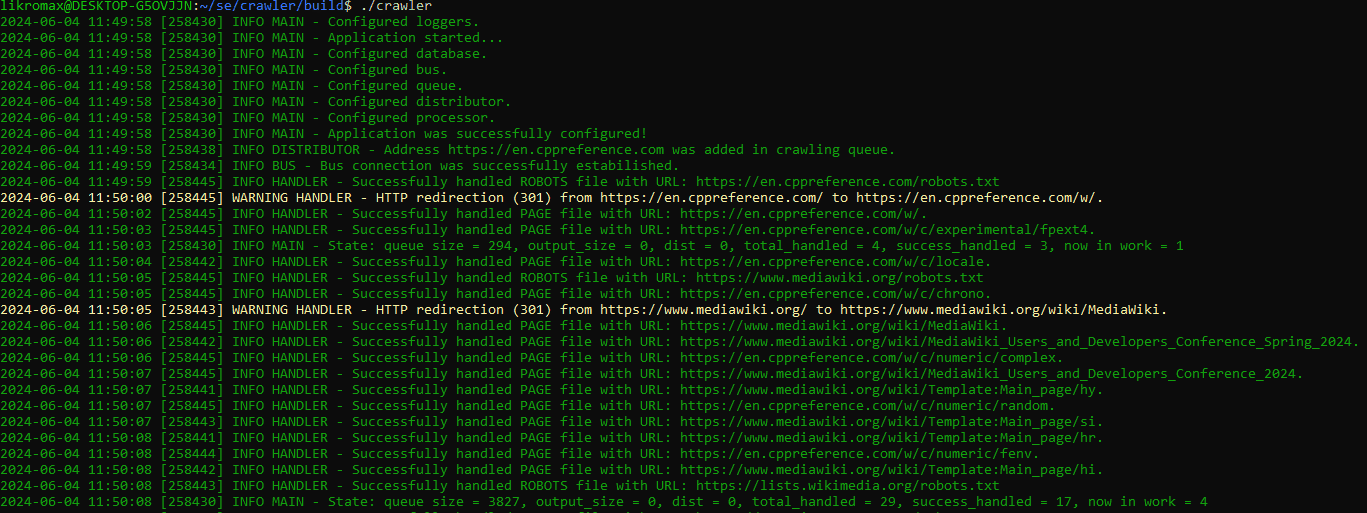
\includegraphics[width=1\linewidth]{tests/robot.png}}
\caption{Информация о промежуточных результатах работы поискового робота}
\label{tests/robot.png:image}
\end{figure}

\subsubsection{Системное тестирование индексатора}
Функция: корректный процесс индексирования документов.

Входные данные: информация о документах из брокера с установленным лимитом документов равным 5. 

Результат: информация об успешном прохождении всех этапов индексирования в консольном журнале (рис. 4.2).

\begin{figure}[H]
\center{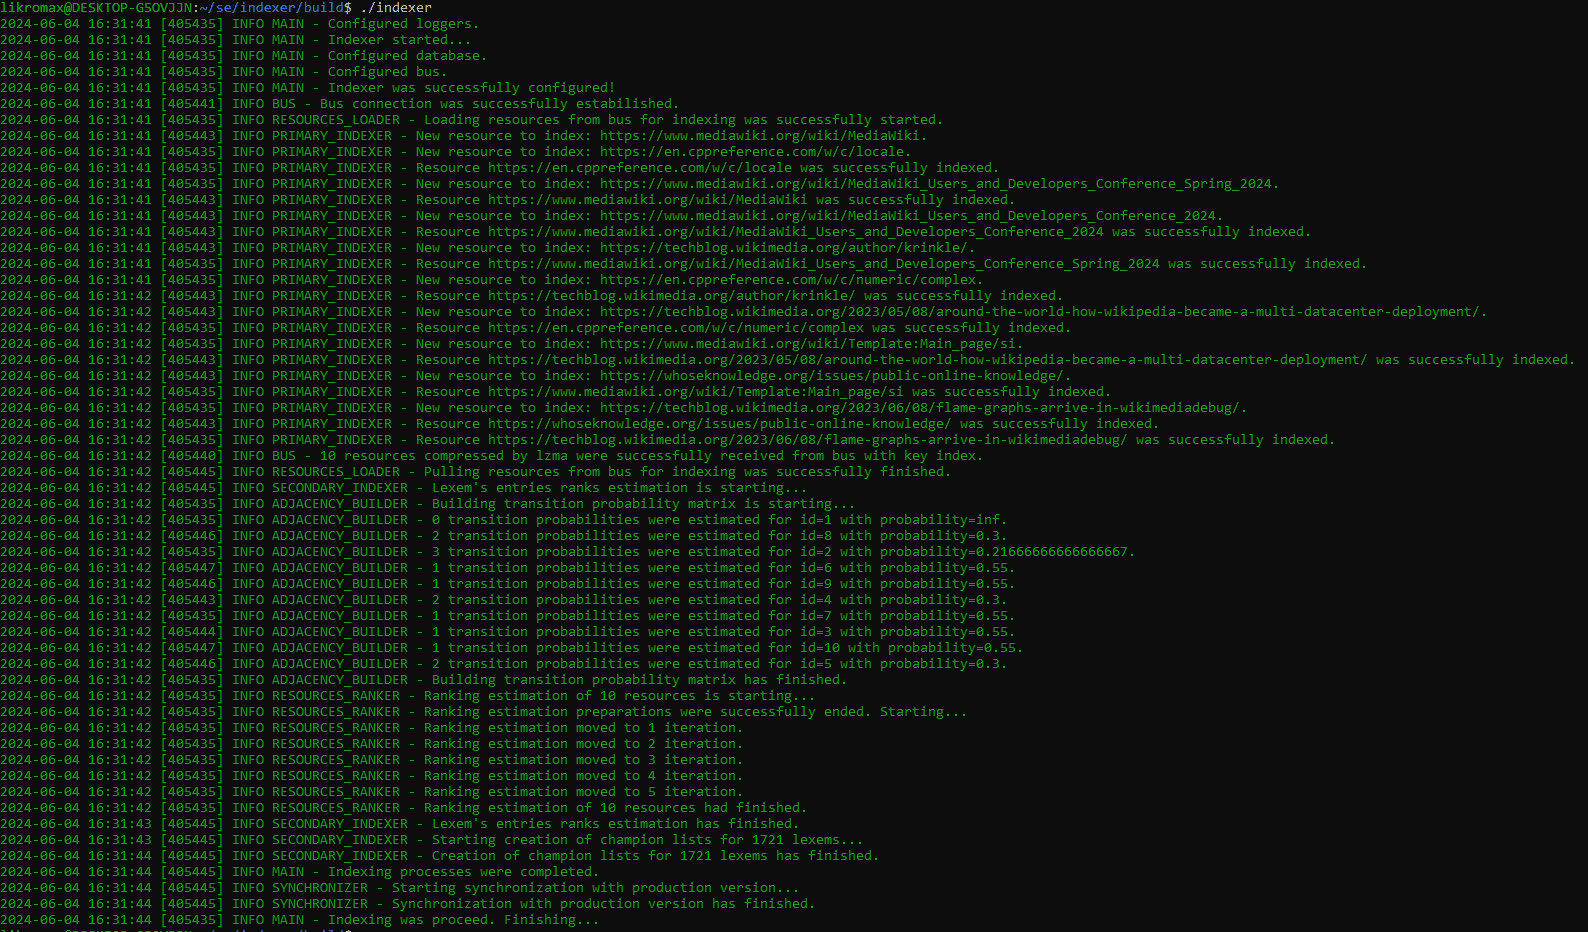
\includegraphics[width=1\linewidth]{tests/indexer.png}}
\caption{Консольная информация об успешном прохождении всех этапов индексирования}
\label{tests/indexer.png:image}
\end{figure}

\subsubsection{Системное тестирование поисковика}

Функция: выдача результатов по пользовательскому запросу.

Входные данные: запрос "<unique ptr"> с нулевым смещением и 10 желаемыми результатами.

Результат: результаты поиска по запросу в программе для тестирования API Postman и информация об успешной работе поисковика в консольном журнале (рис. 4.3 - 4.4).

\begin{figure}[H]
\center{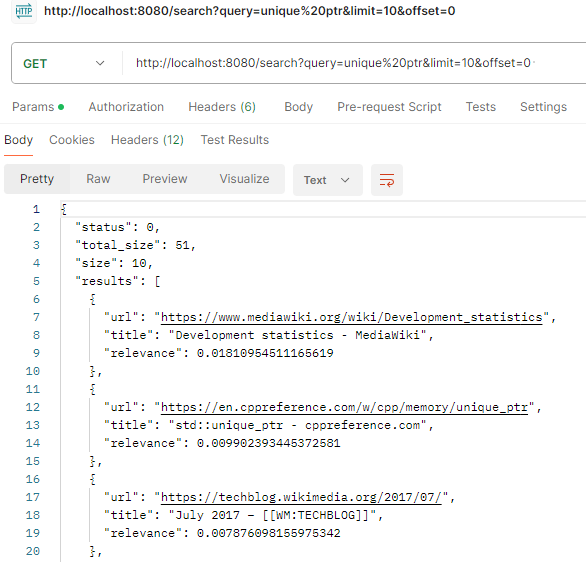
\includegraphics[width=1\linewidth]{tests/searcher_results.png}}
\caption{Фрагмент результатов поиска по запросу "<unique ptr"> в Postman}
\label{tests/searcher_results.png:image}
\end{figure}

\begin{figure}[H]
\center{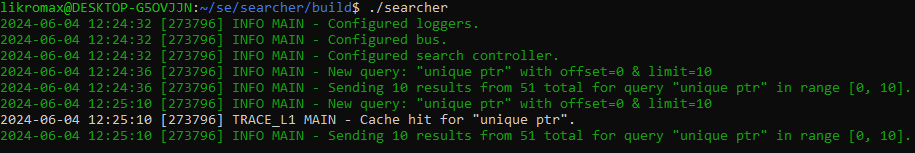
\includegraphics[width=1\linewidth]{tests/searcher_logs.png}}
\caption{Информация консольного журнала о работе поисковика}
\label{tests/searcher_logs.png:image}
\end{figure}

\subsubsection{Системное тестирование сборщика журналируемой информации}

Функция: корректный сбор журналируемой информации.

Входные данные: сообщения из брокера.

Результат: информация об успешном сборе сообщений в консольном журнале (рис. 4.5).

\begin{figure}[H]
\center{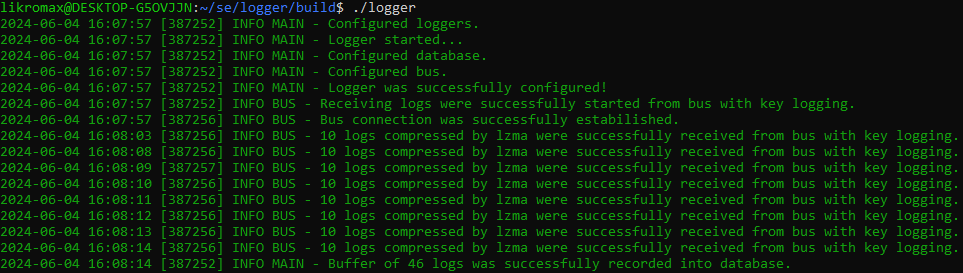
\includegraphics[width=1\linewidth]{tests/logger.png}}
\caption{Консольная информация о сборе журналированных сообщений из брокера}
\label{tests/logger.png:image}
\end{figure}

\subsubsection{Системное тестирование веб-интерфейса}

Функция: отображение результатов поиска по пользовательскому запросу.

Входные данные: запрос "<anna">.

Результат: отображение результатов поиска по запросу (рис. 4.6).

\begin{figure}[H]
\center{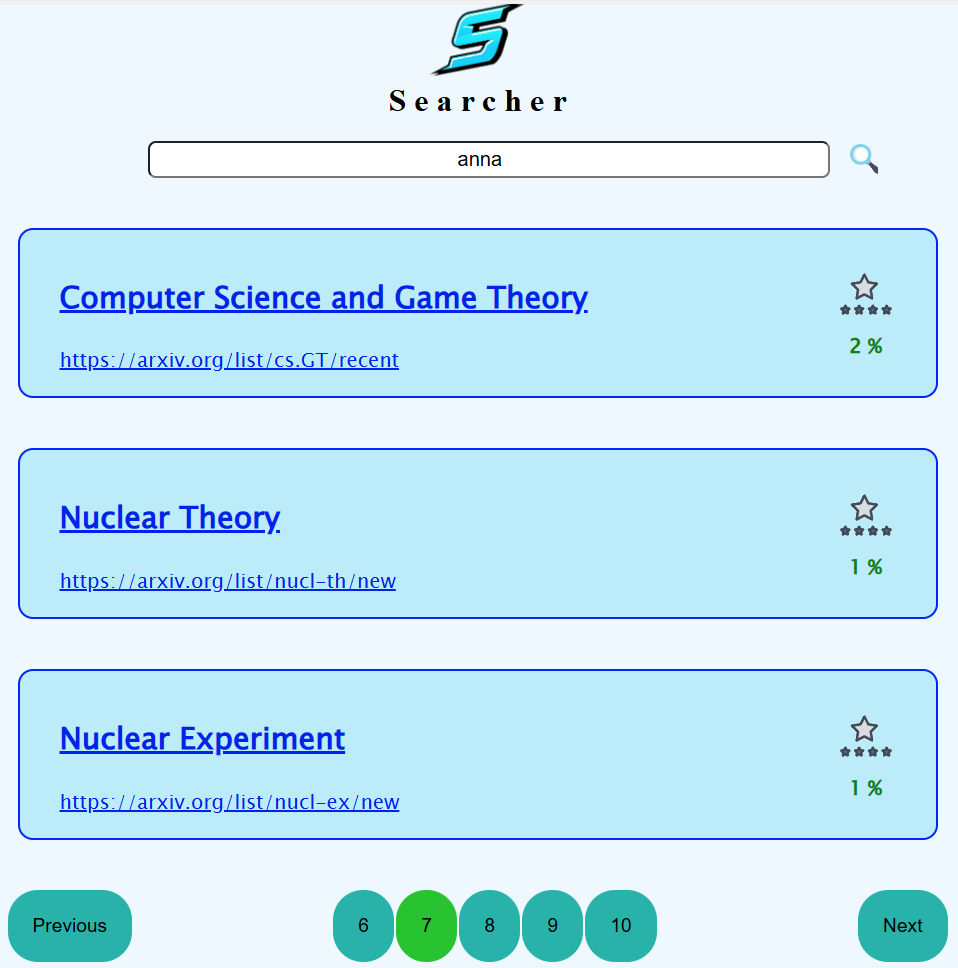
\includegraphics[width=1\linewidth]{tests/web.png}}
\caption{Отображение низкорелевантных результатов поиска по запросу "<anna">}
\label{tests/web.png:image}
\end{figure}